\documentclass{beamer}
\mode<presentation>

\usepackage[english]{babel}
\usepackage[latin1]{inputenc}
\usepackage{times}
\usepackage[T1]{fontenc}
\usepackage{graphicx}
\usepackage[justification=centering]{caption}
\usepackage{subcaption}
\usepackage{url}
\usepackage{setspace}
\usepackage{color}
\usepackage{algorithm2e}

\usepackage{listings}
\lstset{breaklines=true}
%\lstset{upquote=true}
\lstset{basicstyle= \small}%\footnotesize}

\usepackage{tikz}
\usetikzlibrary{trees}

\usepackage{pgfpages}

\addtobeamertemplate{navigation symbols}{}{%
    \usebeamerfont{footline}%
    \usebeamercolor[fg]{footline}%
    \hspace{1em}%
    \insertframenumber%/\inserttotalframenumber
}

\AtBeginSection[]{
  \begin{frame}
  \vfill
  \centering
  \begin{beamercolorbox}[sep=8pt,center,shadow=true,rounded=true]{title}
    \usebeamerfont{title}\insertsectionhead\par%
  \end{beamercolorbox}
  \vfill
  \end{frame}
}

\usepackage{hyperref}

\newcommand{\orka}{\textit{Orka}}
\newcommand{\petra}{\textit{PETrA}}

\newcommand{\monkeyrunner}{\texttt{monkeyrunner}}
\newcommand{\apk}{\texttt{apk}}
\newcommand{\logcat}{\texttt{logcat}}
\newcommand{\netstats}{\texttt{netstats}}

\newcommand{\lv}{Linares-Vasquez et al.}
\setbeameroption{show notes on second screen=right}
%\setbeameroption{show only notes}
%\setbeameroption{show notes}
\title[Project presentation]{\textsc{Hardware usage accounting and source-line level energy estimates on Android}}
\author{Alexandre \textsc{Cornet}\\ {\footnotesize supervised by Dr. Anandha \textsc{Gopalan}}}
\institute{Imperial College London}
\date{September 2017}
\pgfdeclareimage[height=0.5cm]{university-logo}{figures/imperial.pdf}
\logo{\pgfuseimage{university-logo}}
\begin{document}
\tikzstyle{every node}=[draw=black,thick,anchor=west]
\tikzstyle{selected}=[draw=red,fill=red!30]
\tikzstyle{optional}=[dashed,fill=gray!50]
\begin{frame}
\titlepage
\note{extended an energy profiler for Android Applications\\
specifically, focussed on hardware and source line level estimates}
\end{frame}
%
\iffalse
\begin{frame}
\framtitle
\tableofcontents%[pausesections]
}
\end{frame}
\fi
%
%%%%%%%%%%%%%%% PROBLEM
%
\section{Problem}
\note{What problem did I try to solve?\\
App dev doing well\\
But keep getting this}
% FIXME text box on top of frame
\begin{frame}{Energy efficiency matters}
\begin{columns}
\begin{column}{0.5\textwidth}
\begin{figure}
        
\includegraphics[width=\textwidth]{figures/angry_feedback_1.png}
\end{figure}
\end{column}
\begin{column}{0.5\textwidth}
\begin{figure}
        
\includegraphics[width=\textwidth]{figures/angry_feedback_2.png}
\end{figure}
\end{column}
\end{columns}
\note{
angry feedback regarding the energy consumption of your app\\
realize energy eff matters\\
decide to optimise your code for it\\%and to  \alert{find energy bugs}
What are your options?
}
\end{frame}
%
%%%%%%%%%%%%%%% RELATED WORK
%
\section{Related work}
\note{
What's the related work of this project?\\
Best option is definitely to use an energy profiler
}
\begin{frame}{Energy-profilers}
\begin{itemize}
\item Highlight the energy-greediest parts of the code
\item Three types:
\begin{enumerate}
\item hardware-based
\item model-based
\item software-based
\end{enumerate}
\item Yet, \alert{no solution accessible} to the majority of developers
\end{itemize}
\note{
tools which \alert{provide estimates} of the consumption of the code\\
are able to highlight...\\~\\
3 types...\\
hw and model-based rely on \alert{expensive power measurement platforms}\\
financial and practical overhead\\
software-based tools introduced to move away from this requirements\\
however, as this project started, \alert{no publicly available tool}\\~\\
hence \alert{not accessible} to majority
So, what's missing to solve our problem?
}
\end{frame}
%
%
\begin{frame}{What's missing?}
A software-based energy-profiler:
\begin{enumerate}
\item providing hardware-usage and \alert{tail-energy} accounting,
\item providing \alert{source-line level} estimates,
\item available as an \alert{open-sourced} application.
\end{enumerate}
\note{
After the reviewing the state-of-art literature, my opinion was there is a need for...\\
}
\note[item]{
tail-energy is responsible for a \alert{significant fraction} of the drain}
\note[item]{existing profilers highlight the most costly methods\\
but \alert{still the responsibility of the developers} to find the energy}
\note[item]{
despite the many research contributions focussing on ...\\
developers still don't have access to...\\
that's why we \alert{need a common effort} in the community.}
\note[item]{were the aims of my project\\
After reviewing the related work...\\
\alert{extending an existing solution}, namely Orka = option to fulfill them.
}
\end{frame}
%
%%%%%%%%%%%%%%% ORKA
%
\section{Orka}
\note{introduce orka}
\begin{frame}{\orka{}: overview}
\begin{itemize}
%\item Input: Tested \apk{} file and \monkeyrunner{} test script
%\item Output: Energy estimates at the method-level
\item Main assumption:
$$ cost(routine) = \sum_{API \in routine} cost(API)$$
\item Rely on \alert{instrumentation} and on the Android emulator
\end{itemize}
\note{
Based on \alert{LV work}, it approximates\\
Based on this assumption, it \alert{tallies calls} to the A. API\\
Rely on \alert{instrumentation}
}
\end{frame}
%
%
\begin{frame}{\orka{}: workflow}
\begin{figure}
        \includegraphics[width=\textwidth]{figures/orkaworkflow.pdf}
\end{figure}
\note{in and out\\
how does this work?}
\end{frame}
%
%
\begin{frame}
  \vfill
  \centering
  \begin{beamercolorbox}[sep=8pt,center,shadow=true,rounded=true]{title}
    \usebeamerfont{title}Demo\par%
  \end{beamercolorbox}
  \vfill
\note{unlock phone}
\end{frame}
%%%%%%%%%%%%%%% HARDWARE
%
\section{Hardware-usage and tail-energy accounting}
\note{First, define tail energy}
\begin{frame}{Tail-energy}
\note{
definition, how possible?\\
power behaviour can be modelled using a \alert{power state machine}\\
always \alert{two states at least}\\
with or without workflow\\~\\
for many mobile component, a \alert{third state}, the tail-state\\
continue to drain the battery after the workflow has been processed
}
\begin{columns}
\begin{column}{0.5\textwidth}
\begin{itemize}
\item Tail-energy: the component stays in a high power-state \alert{after} processing a workfow.
\end{itemize}
\end{column}
\pause
\begin{column}{0.5\textwidth}
\begin{figure}
	\centering
	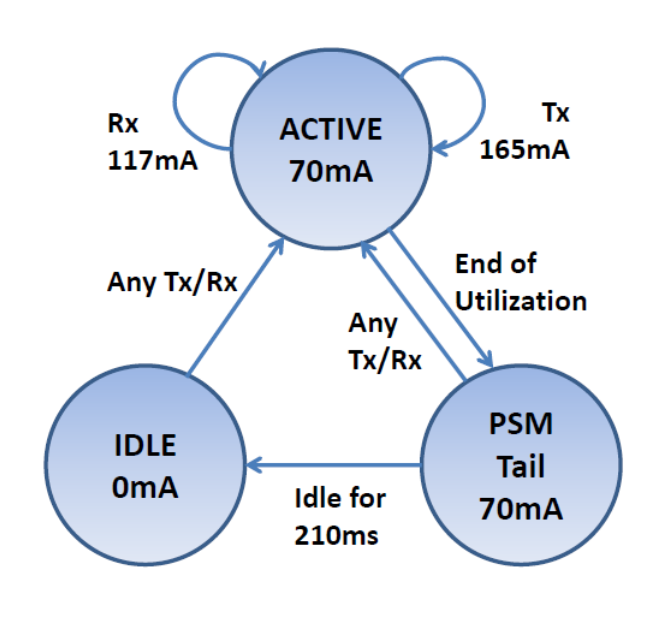
\includegraphics[width=\textwidth]{figures/wifi_statemachine.png} 
	\caption{Power-state machine of a Wi-Fi antenna}
\end{figure}
\end{column}
\end{columns}
\end{frame}
%
%
\begin{frame}{Problem}
\begin{columns}
\begin{column}{0.5\textwidth}
The breakdown by component:
\begin{itemize}
\item is \alert{difficult to interpret},
\item doesn't account for \alert{tail-energy}.
\end{itemize}
\begin{block}{Aims}
\begin{itemize}
\item Map hardware-usage back to the code
\item Account for tail-energy
\end{itemize}
\end{block}
\end{column}
\begin{column}{0.5\textwidth}
\begin{figure}
% FIXME better breakdown
	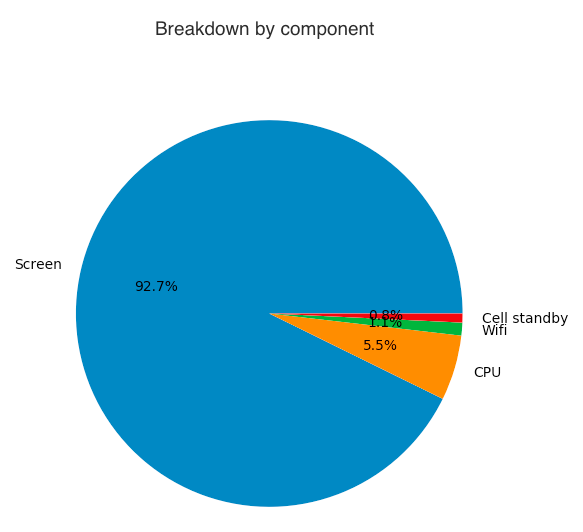
\includegraphics[width=\textwidth]{figures/hw_breakdown.png} 
\end{figure}
\end{column}
\end{columns}
\note{doesn't know what part of the code is responsible for the drain}
\end{frame}
%
%
\begin{frame}[fragile]{Simplifications}
\begin{itemize}
\item Only for Wi-Fi
\item At the method level
\item Focus on time ($E= P \Delta_t$)
\end{itemize}
\begin{block}{Specification}
\begin{itemize}
\item Produce energy tuples
\end{itemize}
\end{block}
\begin{lstlisting}
MainActivity.<init> {ACTIVE: 0.0, IDLE: 0.01,
  TAIL: 0.0}
MainActivity$SendGet.run {ACTIVE: 1.57, IDLE: 0.84,
  TAIL: 1.62}
\end{lstlisting}
\note{
I/O consumes the most energy -- only Wi-FI\\
Simple relation between time and energy -- focus on time\\~\\
Tuples represent the \alert{time spent in each mode } by the Wi-Fi antenna, which is attributed to the method\\
Because of the method XX, the antenna spent ...
}
\end{frame}
%
%
\begin{frame}{Technical challenges}
\begin{block}{Goal}
\begin{itemize}
\item \alert{Correlate} the Wi-Fi energy activity with routine calls
\end{itemize}
\end{block}
\begin{block}{Requirements}
\begin{itemize}
\item Monitoring the call-stack
\item Monitoring the power state of Wi-Fi
\end{itemize}
\end{block}
\note{
call-stack: know which routine are executed at any time\\
Leave call-stack to QA\\~\\

Wifi power state: Not possible to monitor directly as not logged by OS\\
}
\end{frame}
%
%
\begin{frame}[fragile]{Monitoring the power state of Wi-Fi}
% FIXME two col, add state machine
\begin{itemize}
\item We need to monitor what trigger transitions: \alert{network traffic}.
\item Leverage \texttt{proc/net/xt\_qtaguid/stats}
\end{itemize}
\vskip0pt plus.5fill
%[frame=single]
\begin{lstlisting}
idx iface uid_tag_int cnt_set rx_bytes rx_packets tx_bytes tx_packets
2 wlan0 0 0 200888 1096 79636 888
3 wlan0 0 1 0 0 0 0
\end{lstlisting}
\note{
OS log the number of bytes send and received by each application
}
\end{frame}
% FIXME
%
%
\begin{frame}{Implementing the power state-machine}
\begin{figure}
% FIXME better breakdown
	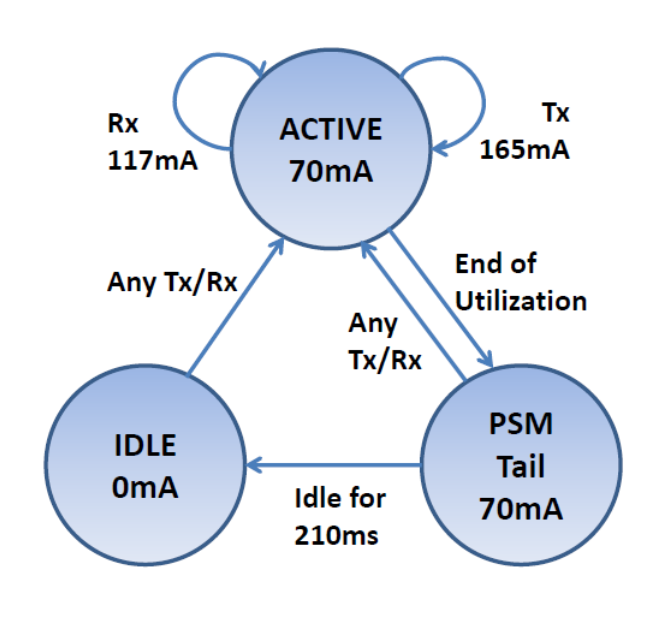
\includegraphics[height=0.6\textheight]{figures/wifi_statemachine.png} 
	\caption{Power-state machine of a Wi-Fi antenna}
\end{figure}
\note{Aim: Deduce Wi-Fi switches from network monitoring\\
leave more detailed speudo QA\\~\\
if any traffic: active\\
no traffic from active: tail\\
if in tail mode: check for time condition
}
\end{frame}
%
% 
\begin{frame}
  \vfill
  \centering
  \begin{beamercolorbox}[sep=8pt,center,shadow=true,rounded=true]{title}
    \usebeamerfont{title}Demo\par%
  \end{beamercolorbox}
  \vfill
\note{git checkout}
\end{frame}
%
%
\begin{frame}[fragile]{Network analyser: principle}
\begin{columns}
\begin{column}{0.5\textwidth}
% 09-04 12:52:26.642 1474 9092 I orka: Ind
\begin{lstlisting}
12:52:26.642 entering foo
12:52:26.742 	...
12:52:26.842 entering bar
12:52:26.942 	...
12:52:27.042 exiting bar
12:52:27.142 exiting foo
\end{lstlisting}
\end{column}
\begin{column}{0.5\textwidth}
\begin{lstlisting}
1503657227.589833 ACTIVE
1503657227.644556 TAIL
1503657227.681700 TAIL
1503657227.716493 TAIL
1503657227.753575 TAIL
1503657227.864556 IDLE
\end{lstlisting}
\end{column}
\end{columns}
\vskip0pt plus.5fill
\begin{itemize}
\item Replay both logs
\item Tally time spent in each mode for all methods
\end{itemize}
\note{
merge sort\\
leave algo for QA\\~\\
let's log processed until t0, state up to date\\
let's fetch next entry at t0 + delta t\\
state is constant during delta t\\
add delta t in current state to all method in the call stack\\
update state\\
loop
}
\end{frame}
%
%
\begin{frame}[fragile]{Network analyser: results}
\begin{lstlisting}
MainActivity.<init> {ACTIVE: 0.0, IDLE: 0.01,
  TAIL: 0.0}
MainActivity$SendGet.run {ACTIVE: 1.57, IDLE: 0.84,
  TAIL: 1.62}
\end{lstlisting}
\end{frame}
%
%%%%%%%%%%%%%%% OTHER WORK
%
\section{Other work}
\note{
other important contributions\\
Important effort were made to \alert{refactor and improve usability}\\
leave to QA
}
%
%
\begin{frame}{Source-line level accounting (1/2)}
\begin{block}{Problem}
\begin{itemize}
\item Method-level estimates highlight costly methods, not energy bugs
\item Developers need even more fine-grained guidance
\end{itemize}
\end{block}
\begin{block}{Implementation}
\begin{itemize}
\item Extended the injector and the traces analyser
\end{itemize}
\end{block}
\end{frame}
%
%
\begin{frame}[fragile]{Source-line level accounting (2/2)}
\centering
%[caption=Example of reconstructed source code providing fine-grained guidance]
{\tiny%\footnotesize
\begin{lstlisting}
method RecList.onCreate, Average cost: 0.0197754308, Calls: 1.0
   2.64% l-1
   1.45% l192 calling RecList.InitRepeatButton
   0.88% l227 calling RecList.InitThemedButtons
   0.57% l229 calling Pref.getPlayingFilePath
  29.04% l247 calling RecList.updateSongList
  21.80% l257 calling android.os.Bundle.getString
  21.80% l258 calling android.os.Bundle.getString
  21.80% l260 calling android.os.Bundle.getString
\end{lstlisting}}
\end{frame}
%
%
\begin{frame}{Evaluation of \orka{}}
TODO
\end{frame}
%
%%%%%%%%%%%%%%% CONCLUSION
%
\section{Conclusion}
\begin{frame}{Summary}
This work stands as the first software-based tool:
\begin{enumerate}
\item accounting for \alert{tail-energy},
\item providing \alert{source-line level} energy estimates,
\item available as an \alert{open-source} application.
\end{enumerate}
\vskip0pt plus.5fill
{\small \orka{} is available at \url{https://github.com/acornet/orka}}
\end{frame}
%
%
\begin{frame}{Future work}
\begin{itemize}
\item Tail-energy: last-trigger policy and extend to other componentss
\item Improve the injector
\item Improve accuracy
\end{itemize}
\end{frame}
%
%
\begin{frame}
  \vfill
  \centering
  \begin{beamercolorbox}[sep=8pt,center,shadow=true,rounded=true]{title}
    \usebeamerfont{title}Thank you\par%
  \end{beamercolorbox}
  \vfill
\end{frame}
%
%%%%%%%%%%%%%%%%%%%%%%%%%%%%%%%%
%
\begin{frame}{Refactoring}
\begin{figure}
\centering
    \begin{subfigure}[b]{0.5\textwidth}
        \centering
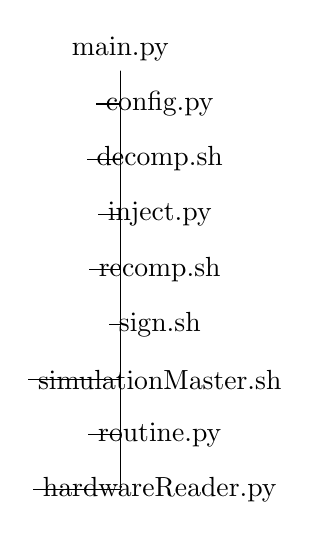
\begin{tikzpicture}[%
  grow via three points={one child at (0.5,-0.7) and
  two children at (0.5,-0.7) and (0.5,-1.4)},
  edge from parent path={(\tikzparentnode.south) |- (\tikzchildnode.west)}]
  \node {main.py}
    child { node {config.py}}
    child { node {decomp.sh}}
    child { node {inject.py}}
    child { node {recomp.sh}}
    child { node {sign.sh}}
    child { node {simulationMaster.sh}}
    child { node {routine.py}}
    child { node {hardwareReader.py}};
\end{tikzpicture}
        \caption{Initial design}
        \label{fig:design:init}
    \end{subfigure}%
    \begin{subfigure}[b]{0.5\textwidth}
        \centering
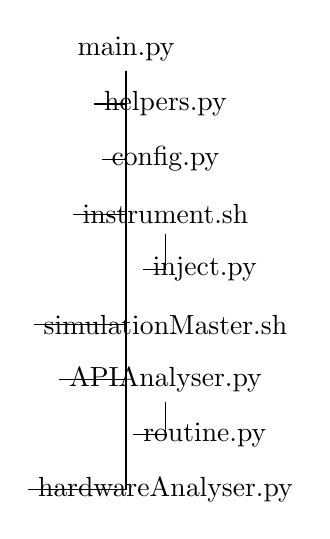
\begin{tikzpicture}[%
  grow via three points={one child at (0.5,-0.7) and
  two children at (0.5,-0.7) and (0.5,-1.4)},
  edge from parent path={(\tikzparentnode.south) |- (\tikzchildnode.west)}]
  \node {main.py}
    child { node {helpers.py}}
    child { node {config.py}}
    child { node {instrument.sh}
    	child { node {inject.py}}}
    child [missing] {}
    child { node {simulationMaster.sh}}
    child { node {APIAnalyser.py}
    	child { node {routine.py}}}
    child [missing] {}
    child { node {hardwareAnalyser.py}};
\end{tikzpicture}
        \caption{New design}
        \label{fig:design:new}
    \end{subfigure}%
\caption{\orka{}'s design}
\label{fig:design}
\end{figure}
\end{frame}
%
%
\begin{frame}[fragile]{Monitoring the call-stack}
\note{
Log when routines start and terminate\\
initial version only log when method enter\\
changed the output format of orka\\
}
\begin{columns}
\begin{column}{0.4\textwidth}
\begin{itemize}
\item Extended the injector to \alert{log when methods return}
\item Used \logcat{} in \texttt{threadtime} mode to \alert{include timestamps}
\end{itemize}
\end{column}
\begin{column}{0.6\textwidth}
% 09-04 12:52:26.642 1474 9092 I orka: Ind
\begin{lstlisting}
12:52:26.642 entering foo
12:52:26.742 	API call api1
12:52:26.842 entering bar
12:52:26.942 	API call api2
12:52:27.042 exiting bar
12:52:27.142 exiting foo
\end{lstlisting}
\end{column}
\end{columns}
\end{frame}
%
%
\begin{frame}{Network monitoring: algorithm}
\begin{small}
\begin{algorithm}[H]
%\KwIn{Active ADB connection to an actual device}
\KwOut{Logs of the energy states of the Wi-Fi antenna}
Get first network statistics $S_0$ at current time $t_0$\;
$state \leftarrow \texttt{IDLE}$\;
\While{True}{
Get network statistics $S_1$ at current time $t_1$\;
\uIf{$S_0 \neq S_1$}
{$state \leftarrow \texttt{ACTIVE}$\;}
\ElseIf{state = \texttt{ACTIVE}}{$state \leftarrow \texttt{TAIL}$\;$tail_{start} \leftarrow t_0$\;}
\If{$state = \texttt{TAIL}$ {\normalfont \textbf{and}} $t_1 - tail_{start} \geq tail_{time}$}
{Log $(t_0, state)$\;
$t_0 \leftarrow tail_{start} + tail_{time}$\;
$state \leftarrow \texttt{IDLE}$\;}
Log $(t_0, state)$\;
$t_0 \leftarrow t_1$, $S_0 \leftarrow S_1$\;
}
\end{algorithm}
\end{small}
\end{frame}
%
%
\begin{frame}[fragile]{Network monitoring: results}
\begin{lstlisting}
1503657227.287407 ACTIVE
1503657227.323574 TAIL
1503657227.359771 TAIL
1503657227.394717 TAIL
1503657227.428777 ACTIVE
1503657227.467203 TAIL
1503657227.518874 ACTIVE
1503657227.589833 ACTIVE
1503657227.644556 TAIL
1503657227.681700 TAIL
1503657227.716493 TAIL
1503657227.753575 TAIL
1503657227.789498 TAIL
1503657227.829724 TAIL
1503657227.864556 IDLE
1503657227.882524 IDLE
\end{lstlisting}
\end{frame}
%
%
\begin{frame}{Network analyser: algorithm}
\begin{small}
\begin{algorithm}[H]
\KwIn{\logcat{} and \netstats{} traces}
\KwOut{Energy tuples describing the Wi-Fi activity for each injected routine}
Initialise routine cost tuples\;
Initialise call stack\;
$state \leftarrow \texttt{IDLE}$\;
\While{{\normalfont Log files contain entries left to process}}{
Get the non-processed entry with the smallest time-stamp\;
Add time spent since the last update in the current state to all routines in the stack\;
Update the call stack if the entry comes from \logcat, otherwise update the $state$\;
}
\end{algorithm}
\end{small}
\note{
let's log processed until t0, state up to date\\
let's fetch next entry at t0 + delta t\\
state is constant during delta t\\
add delta t in current state to all method in the call stack\\
update state\\
loop
}
\end{frame}
%
%
\end{document}
